\documentclass[10pt,twocolumn]{article}

\usepackage{times}
\usepackage{fullpage}

\usepackage{booktabs}  % for \midrule
% \usepackage{subfigure}
% \usepackage{subfig}
\usepackage{balance}
\usepackage{graphicx}
\usepackage{xspace}
\usepackage{subcaption}
%\usepackage{pslatex}
%\usepackage{pifont}
%\usepackage{multirow}
%\usepackage{array}
%\usepackage{booktabs}
%\usepackage{cite}
\usepackage{url}
%\usepackage{cancel}
\usepackage{color,colortbl}
%\usepackage{microtype}
%\usepackage{textcomp}% http://ctan.org/pkg/textcomp
\usepackage{tabularx}
\usepackage{framed}
\usepackage[]{algorithm2e}
\SetAlFnt{\small}
\SetAlCapFnt{\small}
\usepackage{algorithmic}

\usepackage{listings}
%\usepackage{scrextend}
%\usepackage{mathtools}
\usepackage{pbox}

\let\labelindent\relax
\usepackage{enumitem}

\usepackage{tikz}
\usetikzlibrary{arrows,automata}
\usetikzlibrary{calc,positioning}
\usepackage{lipsum,adjustbox}

%\usepackage{tikz}
%\usepackage{decorations.pathmorphing}
%\usepackage{assymb}

\usepackage[labelfont=bf]{caption}

%\theoremstyle{plain}
\newtheorem{theorem}{\bf{Theorem}}%[section]
\newtheorem{lemma}[theorem]{\bf{Lemma}}
\newtheorem{corollary}[theorem]{\bf{Corollary}}
\newtheorem{proofl}[theorem]{\bf{Proof}}
\newtheorem{proposition}[theorem]{\bf{Proposition}}

%\theoremstyle{definition}
\newtheorem{definition}{\bf{Definition}}%[section]
\newtheorem{observation}{\bf{Observation}}%[section] 

%\theoremstyle{remark}
\newtheorem{example}{\bf{Example}}
\newtheorem{notation}{\bf{Notation}}
\newtheorem{fact}{\bf{Fact}}

\usepackage{listings}
%%\usepackage{listings-golang}
\usepackage{color}

%\usepackage{sectsty}
%\sectionfont{\fontsize{12}{15}\selectfont}


\newcommand\mypara[1]{\vspace{.3em}\noindent\textbf{#1}}
\newcommand{\urlwofont}[1]{\urlstyle{same}\url{#1}}


%%%%%%%%%%%%%%%%%%%%%%%%%%%%%%%%%%%%%%%%
% Useful reviewing/feedback annotations
\usepackage{ifthen}
\usepackage[normalem]{ulem} % for \sout
\usepackage{xcolor}
\usepackage{amssymb}

\newcommand{\ra}{$\rightarrow$}
\newboolean{showedits}
\setboolean{showedits}{true} % toggle to show or hide edits
\ifthenelse{\boolean{showedits}}
{
	\newcommand{\ugh}[1]{\textcolor{red}{\uwave{#1}}} % please rephrase
	\newcommand{\ins}[1]{\textcolor{blue}{\uline{#1}}} % please insert
	\newcommand{\del}[1]{\textcolor{red}{\sout{#1}}} % please delete
	\newcommand{\chg}[2]{\textcolor{red}{\sout{#1}}{\ra}\textcolor{blue}{\uline{#2}}} % please change
}{
	\newcommand{\ugh}[1]{#1} % please rephrase
	\newcommand{\ins}[1]{#1} % please insert
	\newcommand{\del}[1]{} % please delete
	\newcommand{\chg}[2]{#2}
}

\newboolean{showcomments}
%\setboolean{showcomments}{true}
\setboolean{showcomments}{false}
\newcommand{\id}[1]{$-$Id: scgPaper.tex 32478 2010-04-29 09:11:32Z oscar $-$}
\newcommand{\yellowbox}[1]{\fcolorbox{gray}{yellow}{\bfseries\sffamily\scriptsize#1}}
\newcommand{\triangles}[1]{{\sf\small$\blacktriangleright$\textit{#1}$\blacktriangleleft$}}
\ifthenelse{\boolean{showcomments}}
%{\newcommand{\nb}[2]{{\yellowbox{#1}\triangles{#2}}}
{\newcommand{\nbc}[3]{
 {\colorbox{#3}{\bfseries\sffamily\scriptsize\textcolor{white}{#1}}}
 {\textcolor{#3}{\sf\small$\blacktriangleright$\textit{#2}$\blacktriangleleft$}}}
 \newcommand{\version}{\emph{\scriptsize\id}}}
{\newcommand{\nbc}[3]{}
 \renewcommand{\ugh}[1]{#1} % please rephrase
 \renewcommand{\ins}[1]{#1} % please insert
 \renewcommand{\del}[1]{} % please delete
 \renewcommand{\chg}[2]{#2} % please change
 \newcommand{\version}{}}
\newcommand{\nb}[2]{\nbc{#1}{#2}{orange}}

\definecolor{ibcolor}{rgb}{0.4,0.6,0.2}
\newcommand\iv[1]{\nbc{IB}{#1}{ibcolor}}
\usepackage{wasysym}
\newcommand\yesml[1]{\nbc{ML {\textcolor{yellow}\sun}}{#1}{mircolor}}

\definecolor{sgcolor}{rgb}{0.2,0.0,0.5}
\newcommand\sg[1]{\nbc{SG}{#1}{sgcolor}}

\definecolor{samcolor}{rgb}{0.2,0.4,0.2}
\newcommand\sam[1]{\nbc{SC}{#1}{samcolor}}

\definecolor{hccolor}{rgb}{0.21,0.54,0.84}
\newcommand\hc[1]{\nbc{HC}{#1}{hccolor}}

% Todo Command
\definecolor{todocolor}{rgb}{0.9,0.1,0.1}
\newcommand{\todo}[1]{\nbc{TODO}{#1}{todocolor}}


%%%%%%%%%%%%%%%%%%%%%%%%%%%%%%%%%%%%%%%%


\begin{document}

%\title{Inferring likely data invariants of distributed systems}
\title{Network Optimized Far Memory}
\author{Stewart Grant \\ University of Califonia San Diego}
\date{}

\maketitle

% \section{Abstract}

\section{Introduction}

My work focuses on the design of algorithms and data
structures for remote memory. I am interested in how
programmable network devices can be integrated into these
systems to provide high performance.
%%
This work is motivated by the observation that the imbalance
between compute and memory capacity for data center servers
has only grown over the past decade while network devices 
are simultaneously faster, and more programmable than ever.
%%
These trends have yielded various research proposals for
expanding per-core memory capacity with fast networks.
Memory disaggregation proposes the addition of pools of far
memory attached over a network to clusters of compute
machines, with the promise that large shared pools will
decrease memory stranding and increase overall memory
utilization.

Latency is the chief challenge in realizing practical memory
disaggregation. Low-latency interconnects such as RDMA over
Ethernet have intra-rack round trip latencies on the order
of 1-2$\mu$s.  In contrast to local memory DRAM access times
of 50-100ns, RDMA latency is a 20x overhead. This disparity
prevents many data structures and system functions from
being deployable with remote memory.

Many existing far-memory systems have found performance
success by porting well isolated and slower subsystems like
page swapping remote memory.  These systems avoid a key
feature of local memory \textit{sharing}. Shared data
structures in remote memory can suffer poor performance when
accessed concurrently.  Both traditional lock-based and
optimistically concurrent data structures suffer abysmal
performance when ported to remote memory. Lock-based
algorithms have inflated critical section sizes due to
round-trip delays, and optimistic approaches suffer from
stale caches under contention, and the increased cost of
reading to synchronize caches. In general, shared structures
are hard to port to remote memory.

%% Todo this is my research statement work hard on it.

A key insight of my work is that many far memory performance
pitfalls are the result of slow serialization mechanisms.
Because remote memory has no colocated CPU's, operations
must be serialized by independent clients. We note that the
network already provides de facto serialization during
transit. Programable elements within the network can
orchestrate algorithm-level serialization at line rate.
With this observation in mind we design shared far memory
systems using programmable devices such as NICs and
switches to accelerate performance.

This research summary covers three projects which illustrate
how these devices can be used to improve optimistic data
structures, lock-based structures, and finally, shared
structures in general.  The first system \textit{Swordbox}
demonstrates that by caching the operations of an optimistic
algorithm on a programmable switch contention can be
entirely removed in network enabling up to 40x improvement
in throughput and 300x reduction in tail latency for
contested workloads. The second project \textit{RCuckoo}
shows how with careful algorithm design and the judicial use
of RDMA features a traditional local memory algorithm can be
ported to remote memory. Finally this work presents an
outline for general data structure design for remote memory
using a programmable switch to remove contention in the
general case.


\section{Optimistic Data Structures}
\begin{figure*}[t!]
    \begin{subfigure}{.33\textwidth}
      \centering
      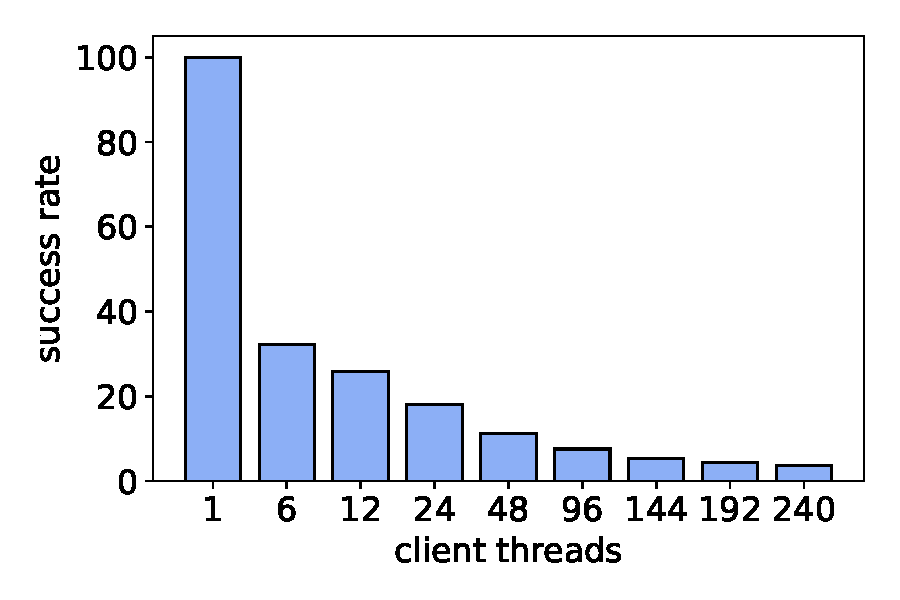
\includegraphics[width=.9\linewidth]{fig/success_rate.pdf}
    \end{subfigure}%
    \begin{subfigure}{.33\textwidth}
      \centering
      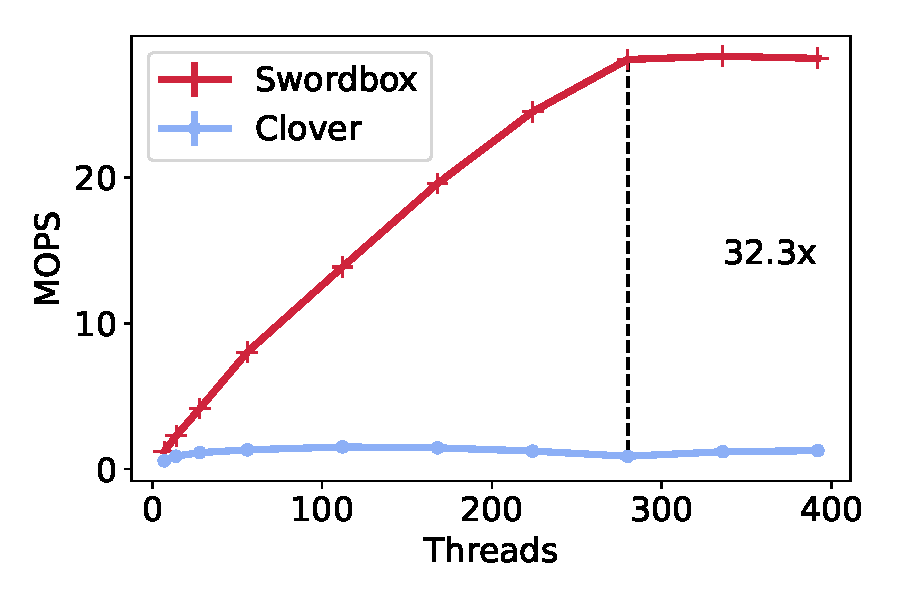
\includegraphics[width=.9\linewidth]{fig/full_system_performance.pdf}
    \end{subfigure}
    \begin{subfigure}{.33\textwidth}
      \centering
      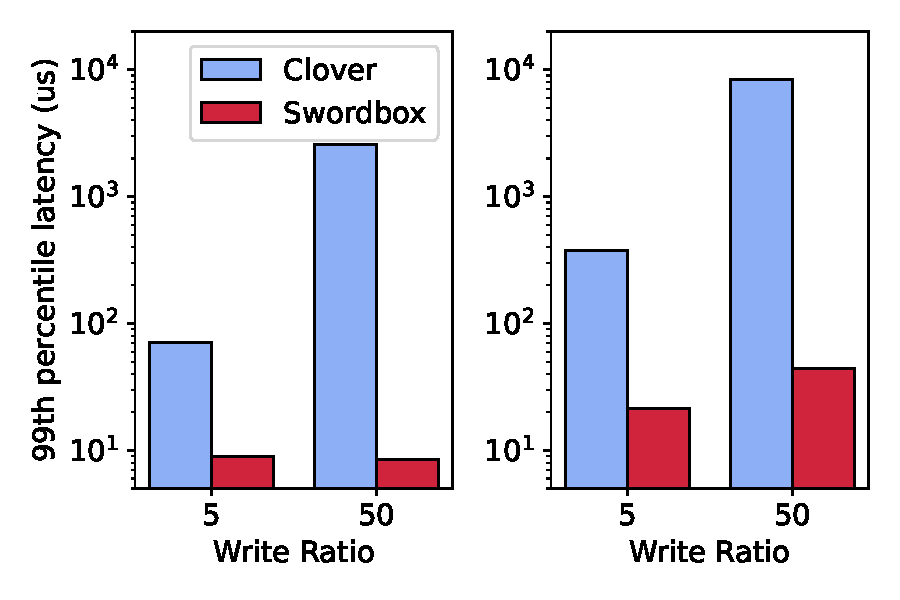
\includegraphics[width=.9\linewidth]{fig/99th_latency.pdf}
    \end{subfigure}

    \caption{Swordbox performance benifits. \textbf{a)} The effect of contention on
    Clover's optimistic writes. \textbf{b)} System throughput
    for YCSB-A (50\% write). \textbf{c)} 99th percentile tail
    latency for different write percentages. Left: read
    latency. Right: write latency}
        
    \label{fig:swordbox}
\end{figure*}

Optimistic concurrency enables high degrees of parallelism
in the absence of contention. At a high level concurrent
processes keep a cache of a shared structure's state, and
then issue operations which succeed if the cache is
synchronized with the shared structure. When memory latency
and contention are high synchronization is difficult as
reads are slower and more expensive, quickly causing local
caches to become stale.

In our work \textit{Swordbox} we make the observation that
at rack-scale the top-of-rack (TOR) switch observes all
remote memory operations in serialized order. This de facto
serialization enables a programmable switch to resolve
conflicting updates to a shared data structure in flight.

In our prototype we resolve optimistic updates to a shared
link list which underpins Clover, a state-of-the-art
disaggregated key value store~\cite{clover}. In Clover keys
are stored as a linked list; when clients update a key they
issue an append to the tail of the list. When keys are under
contention appends to the list frequently fail as the
clients issue appends to stale version of the list's tail.

Figure~\ref{fig:swordbox} a) shows how the success rate of
clovers writes plummets as the number of concurrent clients
increase. When requests fail, clients must issue reads to
the list, find the tail, and execute the write again causing
throughput to drop, and tail latency to dramatically
increase. Swordbox fixes this performance pitfall by caching
the tail pointer of hot keys in a P4 program running on a
programmable TOR. When writes pass through Swordbox it
updates its tail pointer to the list.  When Swordbox sees
stale writes, i.e writes issued to old tail locations, it
rewrites the virtual address of the write to append it to
the tail of the list. This technique enables all contested
requests to succeed while using only a small amount of
switch SRAM (64bits per key). Figure~\ref{fig:swordbox} b,c
shows both the throughput (32x) and latency (300x)
improvements of using Swordbox.

Swordbox demonstrates that optimistic algorithms can be
dramatically improved by caching contested variables in
network. Data structures which require updates to many
locations within a structure may be less amenable to
Swordbox's design as the amount of state required to perform
the updates may be large.

% The future direction for this work
% is to investigate data structure design which enables large
% performance boosts through small amounts of in-network
% caching.


\section{Lock Based Data Structures}

\begin{figure*}[t!]
    \begin{subfigure}{.33\textwidth}
      \centering
      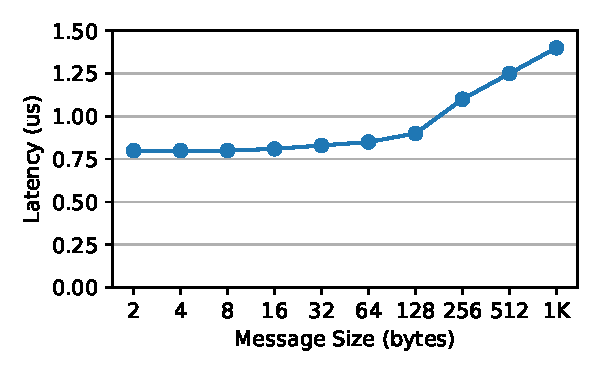
\includegraphics[width=.9\linewidth]{fig/rdma_latency.pdf}
    \end{subfigure}%
    \begin{subfigure}{.33\textwidth}
      \centering
      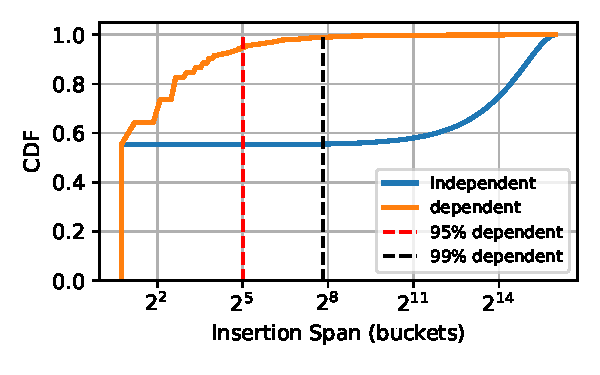
\includegraphics[width=.9\linewidth]{fig/insertion_span.pdf}
    \end{subfigure}
    \begin{subfigure}{.33\textwidth}
      \centering
      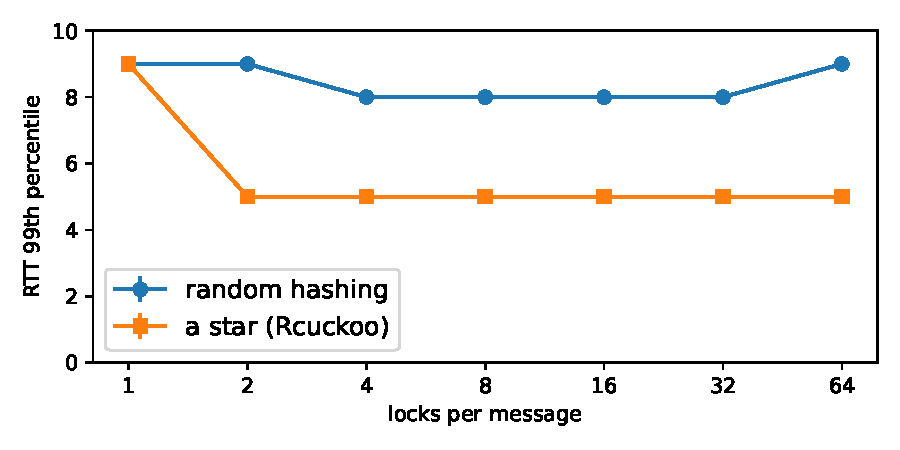
\includegraphics[width=.9\linewidth]{fig/search_dependence.pdf}
    \end{subfigure}

    \caption{RCuckoo algorithmic improvements. \textbf{a)}
    RDMA read latency vs message size. \textbf{b)}RCukoo
    hash locality. The span in table rows which insertions
    span using random hashing vs dependent hashing.
    \textbf{c)} 99th percentile round trips for insertions
    using random hashing vs dependent.}
    \label{fig:rcuckoo}
\end{figure*}


Not all data structures are amenable to oportunistic
updates. Some require extensive updates to a structure where
critical sections provided by traditional locking can
provide a simple way to ensure consistency. Unfortunately,
locks port poorly to remote memory. 
%%
Acquiring and then releasing a lock requires at minimum two
round trips, a fact which not only increases the minimum
operation duration, but which sets a lower bound on
critical-section length. A system with a 2us round-trip time
and a single global lock can only perform 500,000 operations
per second in the best case (meager numbers when considering
that decades-old key value stores acheive 10s of millions of
requests per second~\cite{herd}). Because intra-rack latency
is unlikely to dramatically decrease in the near future,
lock-based remote memory algorithms must be designed to use
fine grained locks. Unfortunately fine grained locking
suffers from a dual problem, deadlock-free lock acquisition
requires a round trip per lock inflating operation time. 

RDMA NICs provide atomic primitives (compare-and-swap) which
can be used to set up to 64 bits (locks) in a single
operation~\cite{melanox-operations}.  Fine grained locking
is therefore a challenge of achieving good lock locality.

With this in mind we investigate porting cuckoo hashing to
remote memory. Cuckoo hashing has long been known to perform
well with RDMA reads as lookups must search at most 2
locations~\cite{pilaf, farm}. The complexity of cuckoo
hashing is pushed to writes which perform swaps randomly
throughout the table. 

%%TODO improve this paragraph
We develop a new system \textit{Rcuckoo} and algorithm for
locality aware cuckoo hashing. Both hash locations of a key
are \textit{likely} to be near one another, rather than in
random locations . Our hash algorithm ensures that with high
probability most pairs of hash locations are close.  This
technique increases the probability that insertions to the
table can be performance with a high degree of locality
within the hash table.

Locality provides many opportunities for network
optimizations. First because both put and get operations are
localized gets can with high likelihood be performed with a
single RDMA read message. Second, because updates are
localized clients can quickly synchronize with the remote
table by issuing a single large RDMA read. These techniques
trade off bandwidth, which is usually plentiful in data
center networks, for latency. Figure~\ref{fig:rcuckoo}a shows
the latency vs packet size tradeoff for RDMA reads. Note that
a packet must be larger than 1024 bytes before issuing two
dependent 64-byte reads is faster than a single large read.

Locality also enables smarter search. Insertions with a
large number of table updates can be slow. Because updates
are localized we can use locality-aware search (e.g. A*) to
quickly find the shortest insertion path.
Figure~\ref{fig:rcuckoo}b shows how A* search and locality
aware hashing (dependent) ensure that 99\% of updates fall
within a 32 row span of the cuckoo table.

Finally and most importantly locality enables efficient
locking. Because updates are localized the locks for a given
set of table updates are likely to be close. We use this
fact, and RDMA masked compare and swap \todo{cite} to
acquire and release all required locks in two round trips in
the average case and five RTT at the 99th percentile.
Figure~\ref{fig:rcuckoo}c, shows the effect of locality on
round trips. On the X-axis the number of locks which are
issued per request is increased. Because of locality RCuckoo
is able to acquire more locks in a single round trip than
random hashing.



As future work we plan to investigate how to modify other
data structures to increase locality.  Prior work on NUMA
optimized, and cache optimized data structures is likely to
yield directly applicable results~\cite{hopscotch}.

\section{General Data Structures}

Swordbox and RCuckoo demonstrate that with careful design
specific optimistic and lock-based data structures can
perform well in remote memory. They do not provide a
general-purpose recipe for designing remote memory data
structures which developers without a deep understanding of
networking and system design can use. In the final work of
my PhD I'm interested in developing such a recipe.

Prior work on NUMA systems has demonstrated that highly
concurrent data structures can be designed in general with a
technique known as \textit{node
replication}~\cite{black-box-numa}. In the node replication
algorithm all operations to a shared structure are made by
appending the operations to a shared log. Clients wishing to
commit operations first read the log, construct the dat
structure locally, and then append to the end of the log
their new operation~\cite{black-box-numa}.

This technique experiences the same contention issues as
Clover in that multiple clients race for the tail of the
list, however on NUMA nodes the memory latency is low enough
that the technique scales well enough for practical
purposes. 

We propose a similar technique for remote memory, with the
addition that a switch, or programmable nic close to memory be
used to remove contention from the shared list. The switch
or NIC can provide two-fold services. The first of which is
to steer appends to the shared list to the end of the list
enabling the success of each client request. Second, using
the fact that large RDMA reads are faster than many
dependent small reads  when clients read the shared log, and
are unaware of the tail location, the switch can inflate the
size of the read in flight by modifying the RDMA read
request. 

Our hope is to demonstrate that pointer-heavy data
structures, and structures with large critical sections such
as linked list, binary trees, and B-trees can be
implemented, and shared in remote memory with good
performance.

\section{Conclusion}

My thesis work focuses on the design and implementation of
shared data structures in disaggregated memory. Using
programmable network technology, we have demonstrated that
both optimistic and lock-based data structures can be
performant. My future research goals aim to generalize these
approaches to reduce developer effort in using remote memory
efficiently.



\balance
\vspace{-0.3cm}
{\footnotesize \bibliographystyle{acm}
\bibliography{paper}}
\vspace{-0.5cm}

\end{document}
